\documentclass{beamer}
\usepackage[utf8]{inputenc}

\usetheme{Madrid}
\usecolortheme{default}
\usepackage{extarrows}
\usepackage{amsmath}
\usepackage{extarrows}
\usepackage{amssymb,amsfonts,amsthm}
\usepackage{txfonts}
\usepackage{tkz-euclide}
\usepackage{listings}
\usepackage{adjustbox}
\usepackage{array}
\usepackage{tabularx}
\usepackage{gvv}
\usepackage{lmodern}
\usepackage{circuitikz}
\usepackage{tikz}
\usepackage{graphicx}
\usepackage{amsmath} 

\setbeamertemplate{page number in head/foot}[totalframenumber]

\usepackage{tcolorbox}
\tcbuselibrary{minted,breakable,xparse,skins}

\definecolor{bg}{gray}{0.95}
\DeclareTCBListing{mintedbox}{O{}m!O{}}{%
  breakable=true,
  listing engine=minted,
  listing only,
  minted language=#2,
  minted style=default,
  minted options={%
    linenos,
    gobble=0,
    breaklines=true,
    breakafter=,,
    fontsize=\small,
    numbersep=8pt,
    #1},
  boxsep=0pt,
  left skip=0pt,
  right skip=0pt,
  left=25pt,
  right=0pt,
  top=3pt,
  bottom=3pt,
  arc=5pt,
  leftrule=0pt,
  rightrule=0pt,
  bottomrule=2pt,
  toprule=2pt,
  colback=bg,
  colframe=orange!70,
  enhanced,
  overlay={%
    \begin{tcbclipinterior}
    \fill[orange!20!white] (frame.south west) rectangle ([xshift=20pt]frame.north west);
    \end{tcbclipinterior}},
  #3,
}
\lstset{
    language=C,
    basicstyle=\ttfamily\small,
    keywordstyle=\color{blue},
    stringstyle=\color{orange},
    commentstyle=\color{green!60!black},
    numbers=left,
    numberstyle=\tiny\color{gray},
    breaklines=true,
    showstringspaces=false,
}
\title %optional
{12.582}
\author 
{EE25BTECH11049-Sai Krishna Bakki}

\begin{document}

\frame{\titlepage}
\begin{frame}{Question}
The position vector $OP$ of point $\vec{P}$ = (20,10) is rotated anti-clockwise in the X-Y plane by an angle $\theta=30^\degree$ such that point $\vec{P}$ occupies position $\vec{Q}$. The coordinates (x,y) of $\vec{Q}$ is 
\end{frame}
\begin{frame}{Theoretical Solution}
   Given
\begin{align}
    \vec{P}=\myvec{20\\10},\theta&=30^\degree
\end{align}
we use
\begin{align}
    \vec{x_n}=\vec{R}\vec{x_o}
\end{align}
where $\vec{R}$ is Rotation matrix
\begin{align}
    \vec{Q}=\myvec{\cos\theta&-\sin\theta\\ \sin\theta&\cos\theta}\vec{P}\\
    \vec{Q}=\myvec{\cos30^\degree&-\sin30^\degree\\ \sin30^\degree&\cos30^\degree}\myvec{20\\10}\\
    \vec{Q}=\myvec{\frac{\sqrt{3}}{2}&\frac{-1}{2}\\\frac{1}{2}&\frac{\sqrt{3}}{2}}\myvec{20\\10}\\
    \vec{Q}=\myvec{10\sqrt{3}-5\\10+5\sqrt{3}}
\end{align}
\end{frame}
\begin{frame}{Theoretical Solution}
Using approximation, the coordinates of $\vec{Q}$ is
\begin{align}
    \vec{Q}=\myvec{12.32\\18.66}
\end{align} 
\end{frame}
\begin{frame}[fragile]
\frametitle{C Code}
\begin{lstlisting}
#include <math.h>
// To ensure M_PI is defined, which is not standard in older C versions
#ifndef M_PI
#define M_PI 3.14159265358979323846
#endif

// Define a structure to hold 2D coordinates.
// This structure will be shared between C and Python.
typedef struct {
    double x;
    double y;
} Point;

void rotate_point_c(Point* p, double angle_degrees) {
    // Convert the angle from degrees to radians for C's math functions
    double angle_radians = angle_degrees * M_PI / 180.0;
\end{lstlisting}
\end{frame}
\begin{frame}[fragile]
\frametitle{C Code}
\begin{lstlisting}
    // Store the original coordinates before overwriting them
    double x_old = p->x;
    double y_old = p->y;

    // Calculate the new coordinates using the standard 2D rotation formulas:
    // x_new = x_old * cos(theta) - y_old * sin(theta)
    // y_new = x_old * sin(theta) + y_old * cos(theta)
    p->x = x_old * cos(angle_radians) - y_old * sin(angle_radians);
    p->y = x_old * sin(angle_radians) + y_old * cos(angle_radians);
}
\end{lstlisting}
\end{frame}
\begin{frame}[fragile]
\frametitle{Python Code Through Shared Output}
\begin{lstlisting}
import ctypes
import os
import matplotlib.pyplot as plt
from matplotlib.patches import Arc
import numpy as np # Required for the plotting function

# Define a Python class that mirrors the C 'Point' struct.
# This tells ctypes how to interpret the block of memory.
class Point(ctypes.Structure):
    _fields_ = [("x", ctypes.c_double),
                ("y", ctypes.c_double)]

def plot_rotation(p, q, angle_degrees):
    """
    Generates a plot to visualize the rotation of point P to Q.
    Args:
        p (tuple): The original (x, y) coordinates.
        q (tuple): The rotated (x, y) coordinates.
        \end{lstlisting}
\end{frame}
\begin{frame}[fragile]
\frametitle{Python Code Through Shared Output}
\begin{lstlisting}
        angle_degrees (float): The angle of rotation.
    """
    fig, ax = plt.subplots(figsize=(8, 8))

    # Plot origin
    ax.plot(0, 0, 'ko', markersize=10, label='Origin (O)')

    # Create formatted strings for the labels
    p_label = f'({p[0]:.2f}, {p[1]:.2f})'
    q_label = f'({q[0]:.2f}, {q[1]:.2f})'

    # Plot vectors and points
    # Vector OP
    ax.arrow(0, 0, p[0], p[1], head_width=0.5, head_length=0.7, fc='blue', ec='blue', length_includes_head=True)
    ax.plot(p[0], p[1], 'bo', markersize=8, label=f'Point P {p_label}')
    ax.text(p[0] + 0.5, p[1] + 0.5, f'P {p_label}', fontsize=12, color='blue')
\end{lstlisting}
\end{frame}
\begin{frame}[fragile]
\frametitle{Python Code Through Shared Output}
\begin{lstlisting}
    # Vector OQ
    ax.arrow(0, 0, q[0], q[1], head_width=0.5, head_length=0.7, fc='red', ec='red', length_includes_head=True)
    ax.plot(q[0], q[1], 'ro', markersize=8, label=f'Point Q {q_label}')
    ax.text(q[0] + 0.5, q[1] + 0.5, f'Q {q_label}', fontsize=12, color='red')

    # Add the rotation arc
    radius = np.linalg.norm(p)
    angle_p_rad = np.arctan2(p[1], p[0])
    angle_p_deg = np.degrees(angle_p_rad)
    arc = Arc((0, 0), radius*0.5, radius*0.5, angle=0,
              theta1=angle_p_deg, theta2=angle_p_deg + angle_degrees,
              color='green', linewidth=2, linestyle='--')
    ax.add_patch(arc)
    theta_label_rad = np.radians(angle_p_deg + angle_degrees / 2)
    \end{lstlisting}
\end{frame}
\begin{frame}[fragile]
\frametitle{Python Code Through Shared Output}
\begin{lstlisting}
    ax.text(radius*0.3 * np.cos(theta_label_rad), radius*0.3 * np.sin(theta_label_rad),
            f'θ={angle_degrees}°', fontsize=12, color='green')

    # Set up the plot aesthetics
    ax.axhline(0, color='black',linewidth=0.5)
    ax.axvline(0, color='black',linewidth=0.5)
    ax.grid(True, which='both', linestyle='--', linewidth=0.5)
    ax.set_aspect('equal', adjustable='box')
    ax.set_title('2D Vector Rotation (using C function)', fontsize=16)
    ax.set_xlabel('X-axis', fontsize=12)
    ax.set_ylabel('Y-axis', fontsize=12)
    max_val = max(abs(p[0]), abs(p[1]), abs(q[0]), abs(q[1])) * 1.2
    ax.set_xlim(-5, max_val)
    ax.set_ylim(-5, max_val)
    ax.legend()
    plt.show()
\end{lstlisting}
\end{frame}
\begin{frame}[fragile]
\frametitle{Python Code Through Shared Output}
\begin{lstlisting}
# --- Main execution block ---
if __name__ == "__main__":
    # Determine the correct shared library file extension based on the operating system
    if os.name == 'nt': # For Windows
        lib_name = 'rotate_vector.dll'
    else: # For Linux, macOS, etc.
        lib_name = 'rot.so'
    
    # Construct the full path to the library file, assuming it's in the same directory
    lib_path = os.path.join(os.path.dirname(os.path.abspath(__file__)), lib_name)

    try:
        # Load the compiled C code as a shared library
        c_lib = ctypes.CDLL(lib_path)
    except OSError as e:
        print(f"Error: Could not load the shared library '{lib_name}'.")
        \end{lstlisting}
\end{frame}
\begin{frame}[fragile]
\frametitle{Python Code Through Shared Output}
\begin{lstlisting}
        print(f"Details: {e}")
        print("\nPlease compile the C code first. See README.md for instructions.")
        exit()

    # Get a handle to the 'rotate_point_c' function inside the library
    rotate_point_c = c_lib.rotate_point_c
    
    # Define the function's signature for ctypes
    rotate_point_c.argtypes = [ctypes.POINTER(Point), ctypes.c_double]
    rotate_point_c.restype = None
# --- Use the C function ---
    p = Point(x=20.0, y=10.0)
    theta = 30.0
    # Store the original coordinates before they are modified, for plotting
    p_original_coords = (p.x, p.y)
\end{lstlisting}
\end{frame}
\begin{frame}[fragile]
\frametitle{Python Code Through Shared Output}
\begin{lstlisting}
    print(f"Original point P: ({p.x}, {p.y})")
    print(f"Rotation angle: {theta}°")
    
    # Call the C function. This modifies the 'p' object in place.
    rotate_point_c(ctypes.byref(p), theta)

    # Store the new coordinates for printing and plotting
    q_rotated_coords = (p.x, p.y)

    print(f"New point Q (calculated by C): ({q_rotated_coords[0]:.2f}, {q_rotated_coords[1]:.2f})")

    # --- Visualize the result ---
    plot_rotation(p_original_coords, q_rotated_coords, theta)
    \end{lstlisting}
\end{frame}
\begin{frame}[fragile]
\frametitle{Python Code}
\begin{lstlisting}
import numpy as np
import matplotlib.pyplot as plt
from matplotlib.patches import Arc

def rotate_point(point, angle_degrees):
    """
    Rotates a 2D point anti-clockwise around the origin.

    Args:
        point (tuple or list): The (x, y) coordinates of the point to rotate.
        angle_degrees (float): The angle of rotation in degrees.

    Returns:
        numpy.ndarray: The new (x, y) coordinates after rotation.
    """
    # Convert the angle from degrees to radians for trigonometric functions
    angle_radians = np.radians(angle_degrees)
\end{lstlisting}
\end{frame}
\begin{frame}[fragile]
\frametitle{Python Code}
\begin{lstlisting}
    # Define the initial point P as a column vector (2x1 matrix)
    p_vector = np.array([[point[0]], [point[1]]])

    # Create the 2D anti-clockwise rotation matrix
    cos_theta = np.cos(angle_radians)
    sin_theta = np.sin(angle_radians)
    rotation_matrix = np.array([
        [cos_theta, -sin_theta],
        [sin_theta,  cos_theta]
    ])

    # Perform the matrix multiplication: Q = R * P
    q_vector = np.dot(rotation_matrix, p_vector)

    return q_vector.flatten() # Flatten to a 1D array for easier reading

def plot_rotation(p, q, angle_degrees):
\end{lstlisting}
\end{frame}
\begin{frame}[fragile]
\frametitle{Python Code}
\begin{lstlisting}
    """
    Generates a plot to visualize the rotation of point P to Q.
    """
    fig, ax = plt.subplots(figsize=(8, 8))

    # Plot origin
    ax.plot(0, 0, 'ko', markersize=10, label='Origin (O)')

    # Create formatted strings for the labels to ensure clean output
    p_label = f'({p[0]:.2f}, {p[1]:.2f})'
    q_label = f'({q[0]:.2f}, {q[1]:.2f})'

    # Plot vectors and points
    # Vector OP
    ax.arrow(0, 0, p[0], p[1], head_width=0.5, head_length=0.7, fc='blue', ec='blue', length_includes_head=True)
    ax.plot(p[0], p[1], 'bo', markersize=8, label=f'Point P {p_label}')
    \end{lstlisting}
\end{frame}
\begin{frame}[fragile]
\frametitle{Python Code}
\begin{lstlisting}
    ax.text(p[0] + 0.5, p[1] + 0.5, f'P {p_label}', fontsize=12, color='blue')
    # Vector OQ
    ax.arrow(0, 0, q[0], q[1], head_width=0.5, head_length=0.7, fc='red', ec='red', length_includes_head=True)
    ax.plot(q[0], q[1], 'ro', markersize=8, label=f'Point Q {q_label}')
    ax.text(q[0] + 0.5, q[1] + 0.5, f'Q {q_label}', fontsize=12, color='red')

    # Add the rotation arc
    radius = np.linalg.norm(p)
    # Angle for arc starts from the angle of vector P
    angle_p_rad = np.arctan2(p[1], p[0])
    angle_p_deg = np.degrees(angle_p_rad)
    arc = Arc((0, 0), radius*0.5, radius*0.5, angle=0,
              theta1=angle_p_deg, theta2=angle_p_deg + angle_degrees,
              color='green', linewidth=2, linestyle='--')
              \end{lstlisting}
\end{frame}
\begin{frame}[fragile]
\frametitle{Python Code}
\begin{lstlisting}
    ax.add_patch(arc)
    # Add theta label near the arc
    theta_label_rad = np.radians(angle_p_deg + angle_degrees / 2)
    ax.text(radius*0.3 * np.cos(theta_label_rad), radius*0.3 * np.sin(theta_label_rad),
            f'θ={angle_degrees}°', fontsize=12, color='green')

    # Set up the plot
    ax.axhline(0, color='black',linewidth=0.5)
    ax.axvline(0, color='black',linewidth=0.5)
    ax.grid(True, which='both', linestyle='--', linewidth=0.5)
    ax.set_aspect('equal', adjustable='box')
    ax.set_title('2D Vector Rotation', fontsize=16)
    ax.set_xlabel('X-axis', fontsize=12)
    ax.set_ylabel('Y-axis', fontsize=12)

    # Set axis limits to give some space around the vectors
    max_val = max(np.abs(p).max(), np.abs(q).max()) * 1.2
    \end{lstlisting}
\end{frame}
\begin{frame}[fragile]
\frametitle{Python Code}
\begin{lstlisting}
    ax.set_xlim(-5, max_val)
    ax.set_ylim(-5, max_val)
    ax.legend()
    plt.show()

# --- Main execution ---
if __name__ == "__main__":
    # Initial point P
    P = np.array([20, 10])

    # Angle of rotation in degrees
    theta = 30

    # Calculate the new position Q
    Q = rotate_point(P, theta)
    print(f"Original point P: {tuple(P)}")
    print(f"Rotation angle: {theta}°")
    print(f"New point Q (x, y): ({Q[0]:.2f}, {Q[1]:.2f})")
    plot_rotation(P, Q, theta)
\end{lstlisting}
\end{frame}
\begin{frame}{Plot By C code and Python Code}
    \begin{figure}
    \centering
    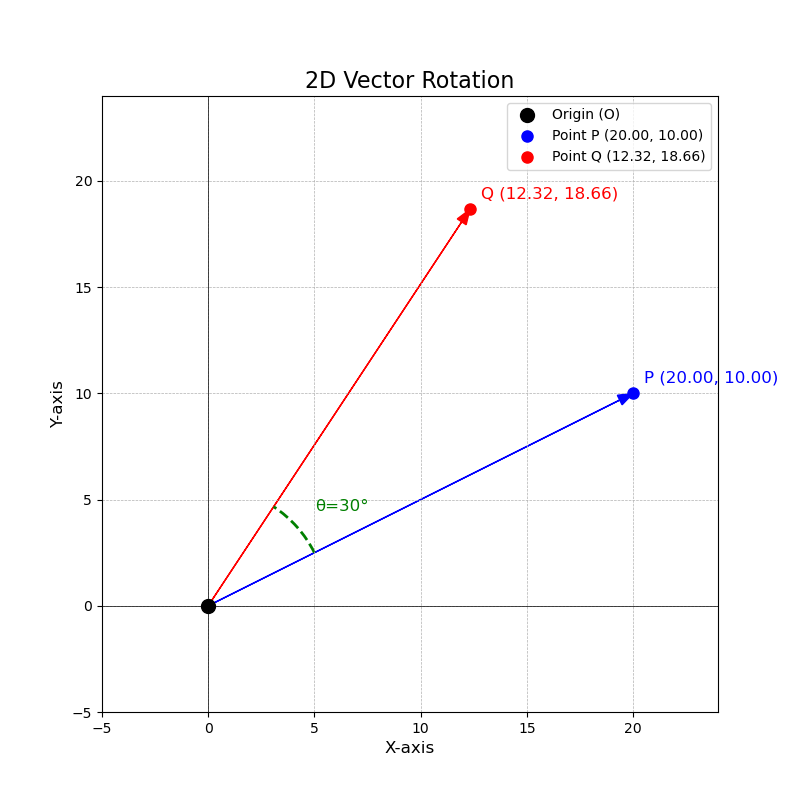
\includegraphics[width=0.7\columnwidth]{figs/Figure_1.png}
    \label{fig:placeholder}
    \caption{1}
\end{figure}
\end{frame}
\end{document}
